\documentclass[GBK,UTF8,12pt,oneside,a4paper]{ctexbook}
%----------------------------------------packages and format-----------------
%\input{setup/package.tex}
\usepackage{xtuformat}
\graphicspath{{figures/}}
\usepackage{fancyhdr}
\usepackage{gbt7714}
\usepackage{subfigure}
\usepackage[subfigure]{tocloft}
\usepackage{setspace}
\usepackage{mathtools}
\usepackage{natbib}
\usepackage{caption}
%\usepackage{newtxmath}
\usepackage{pifont}
\usepackage[perpage,symbol*,hang,flushmargin]{footmisc}
\usepackage{dirtree}
\usepackage{tabularray}
\usepackage{listings}
\lstset{
	language=Python, % 设置语言
	basicstyle=\ttfamily, % 设置字体族
	breaklines=true, % 自动换行
	keywordstyle=\bfseries\color{NavyBlue}, % 设置关键字为粗体,颜色为 NavyBlue
	morekeywords={}, % 设置更多的关键字,用逗号分隔
	emph={self}, % 指定强调词,如果有多个,用逗号隔开
	emphstyle=\bfseries\color{Rhodamine}, % 强调词样式设置
	commentstyle=\itshape\color{black!50!white}, % 设置注释样式,斜体,浅灰色
	stringstyle=\bfseries\color{PineGreen!90!black}, % 设置字符串样式
	columns=flexible,
	numbers=left, % 显示行号在左边
	numbersep=2em, % 设置行号的具体位置
	numberstyle=\footnotesize, % 缩小行号
	frame=single, % 边框
	framesep=1em % 设置代码与边框的距离
}

\bibliographystyle{gbt7714-numerical}

\renewcommand\theequation{\arabic{chapter}-\arabic{equation}}

\renewcommand {\thetable} {\thechapter{}-\arabic{table}}
\renewcommand {\thefigure} {\thechapter{}-\arabic{figure}}
\DeclareCaptionFont{cap}{\songti\bfseries\zihao{5}}

\newtagform{dots}{$\cdots$\ (}{)}%

\DefineFNsymbols{circled}{{\ding{192}}{\ding{193}}{\ding{194}}
{\ding{195}}{\ding{196}}{\ding{197}}{\ding{198}}{\ding{199}}{\ding{200}}{\ding{201}}}
\setfnsymbol{circled}

\renewcommand{\footnotesize}{\songti\zihao{-5}}

\begin{document}
%----------------------------------------setup-----------------------
\captionsetup{font={cap},labelfont={cap},labelformat=default,labelsep=space}
%设置全文页眉、页脚的格式
\pagestyle{fancy}
\fancypagestyle{plain}{
\pagestyle{fancy}
}
\renewcommand{\headrulewidth}{0pt}
\lhead{}           %页眉左边设为空
\chead{\zihao{5}湘潭大学毕业论文}           %页眉中间
\rhead{}           %页眉右边
%\rhead{\includegraphics[width=1.2cm]{1.eps}}  %页眉右侧放置logo
\lfoot{}          %页脚左边
%\cfoot{}  %页脚中间
\rfoot{}          %页脚右边

\pagenumbering{Roman}
%插入摘要
%----摘要----------------------------------------------------------------------------------------
\phantomsection\addcontentsline{toc}{chapter}{摘要}\tolerance=500 %将摘要放进目录
\begin{cnabstract}
本文介绍湘潭大学论文模板 的使用方法。本模板符合学校的本科论文格式要求。

摘要二字中间空两个汉字空格或4个半角空格,中文字体为宋体,西文字体为Times New Roman,三号,加粗,大纲级别1级,居中无缩进,段前0行,段后0行,单倍行距。另起一页。

摘要内容为中文字体为宋体,西文字体为Times New Roman,五号,大纲级别正文文本,两端对齐,首行缩进2字符,段前0.5行,段后0.5行,固定值20磅。

“关键词:”宋体小四号加粗,其后关键词中文字体为宋体,西文字体为Times New Roman,五号,大纲级别正文文本,两端对齐,首行缩进2字符,段前0行,段后0行,固定值20磅。每一关键词之间用全角分号隔开(;)最后一个关键词后不打标点符号。关键词前空一空白行。
\end{cnabstract}
~\par
\begin{cnkeywords}
关键词1;关键词2
\end{cnkeywords}
%----Abstract------------------------------------------------------------------------------------
\newpage
\phantomsection\addcontentsline{toc}{chapter}{Abstract}\tolerance=500 %将摘要放进目录
\begin{enabstract}
This article introduces how to use the thesis template of Xiangtan University. This template complies with the university's undergraduate dissertation formatting requirements.

There should be two Chinese character spaces or 4 half-width spaces in the middle of the word abstract. The Chinese font is Times New Roman, and the Western font is Times New Roman, size 3, bold, outline level 1, centered without indentation, 0 lines before a paragraph, paragraph After 0 lines, single line spacing. Start another page.

The content of the abstract is Song typeface in Chinese, Times New Roman in Western font, size 5, outline-level body text, justified, 2 characters indentation for the first line, 0.5 lines before a paragraph, 0.5 lines after a paragraph, and a fixed value of 20 points.

"Keywords:" Song Ti small four bold, followed by the Chinese font is Song Ti, Western font is Times New Roman, five, outline level body text, justified at both ends, the first line indented 2 characters, before the paragraph 0 lines, 0 lines after the paragraph, fixed value 20 points. Separate each keyword with a full-width semicolon (;) without a punctuation mark after the last keyword. There is a blank line before the keywords.
\end{enabstract}
~\par
\begin{enkeywords}
keyword1; keyword2
\end{enkeywords} 

%----------------------------------------table content-----------------------
\newpage

\renewcommand{\contentsname}{\centerline{\songti\zihao{3}\bfseries{目\quad\quad 录}}}
\renewcommand{\cftchapleader}{\cftdotfill{0.6}}
\renewcommand{\cftsecleader}{\cftdotfill{0.6}}
\renewcommand{\cftsubsecleader}{\cftdotfill{0.6}}
\renewcommand{\cftchapfont}{\songti\zihao{4}}
\renewcommand{\cftchappagefont}{\songti\zihao{4}}
\renewcommand{\cftsecfont}{\songti\zihao{-4}}
\renewcommand{\cftsecpagefont}{\songti\zihao{-4}}
\renewcommand{\cftsubsecfont}{\songti\zihao{-4}}
\renewcommand{\cftsubsecpagefont}{\songti\zihao{-4}}
\setlength\cftbeforechapskip{0.4\baselineskip}
\setlength\cftbeforesecskip{0.4\baselineskip}
\setlength\cftbeforesubsecskip{0.4\baselineskip}
\setlength{\cftbeforetoctitleskip}{24pt}
\setlength{\cftaftertoctitleskip}{18pt}
\tableofcontents



%----------------------------------------bodypre--------------------------------
\CTEXsetup[format={\songti\bfseries\zihao{3}},name={},number={\arabic{chapter}}]{chapter}
\CTEXsetup[beforeskip={24pt},afterskip={18pt}]{chapter}
\songti\zihao{-4}
\setlength{\baselineskip}{20pt}
% 从第一章开始用阿拉伯数字编号
\newpage
\pagenumbering{arabic}
%----------------------------------------body--------------------------------
\chapter{绪论}\label{chap:introduction}
目录二字中间空两个汉字空格或4个半角空格,目录显示到三级标题,四级及以后均不显示。目录中需包含摘要和Abstract。目录标题宋体,三号,加粗,居中无缩进,段前24磅,段后18磅,固定值20磅。大纲级别正文文本。另起一页。
一级目录项:中文字体为宋体,西文字体为Times New Roman,四号,两端对齐,首行无缩进,左缩进0字符,右缩进0字符,段前0行,段后0行,1.5倍行距。
二级目录项:中文字体为宋体,西文字体为Times New Roman,小四号,两端对齐,首行无缩进,左缩进2字符,右缩进0字符,段前0行,段后0行,1.5倍行距。
三级目录项:中文字体为宋体,西文字体为Times New Roman,小四号,两端对齐,首行无缩进,左缩进4字符,右缩进0字符,段前0行,段后0行,1.5倍行距。
注意保持页码右对齐,有前导符,正文修改后注意刷新目录保持一致。目录中的摘要,附录,致谢,均不要空格。

\section{标题}
正文另起一页,一级标题:中文字体为宋体,西文字体为Times New Roman,三号,加粗,大纲级别1级,两端对齐,首行无缩进,段前24磅,段后18磅,固定值20磅。题序与标题间空1格。

二级标题:中文字体为宋体,西文字体为Times New Roman,四号,加粗,大纲级别2级,两端对齐,首行无缩进,段前24磅,段后6磅,固定值20磅。题序与标题间空1格。

正文:中文字体为宋体,西文字体为Times New Roman,小四号,大纲级别正文文本,两端对齐,首行缩进2字符,段前0行,段后0行,固定值20磅。

脚注:中文字体为宋体,西文字体为Times New Roman,小五号,左对齐,无缩进,段前0行,段后0行,单倍行距。每页重新编号,编号方式为\footnote{脚注1}

\subsection{标题}
三级标题:中文字体为宋体,西文字体为Times New Roman,小四号,加粗,大纲级别3级,两端对齐,首行无缩进,段前12磅,段后6磅,固定值20磅。题序与标题间空1格。
\subsubsection{标题}
四级标题:中文字体为宋体,西文字体为Times New Roman,小四号,大纲级别4级,两端对齐,首行无缩进,段前6磅,段后6磅,固定值20磅。题序与标题间空1格。

参考文献引用\upcite{Arteaga-Falconi:ITIM:2016}\upcite{Barni:ITIFS:2011}
\upcite{Dautov:IJBHI:2016,Hartley:ITITB:2012,Hu:ITITB:2007}。
\chapter{图表,伪代码,公式相关排版}\label{elements}

\section{图的排版}
图题:中文字体为宋体,西文字体为Times New Roman,五号,加粗,居中无缩进,段前6磅,段后12磅,单倍行距。图名在图号之后空一格排写。图名后不加标点符号。

图注或图片来源说明:中文字体为宋体,西文字体为Times New Roman,小五号,两端对齐,首行缩进2字符,段前0行,段后0行,固定值20磅。

\subsection{单图}
单图排版。

\begin{figure}[!htb]
\centering
\begin{minipage}[t]{\oneimage}
\centering
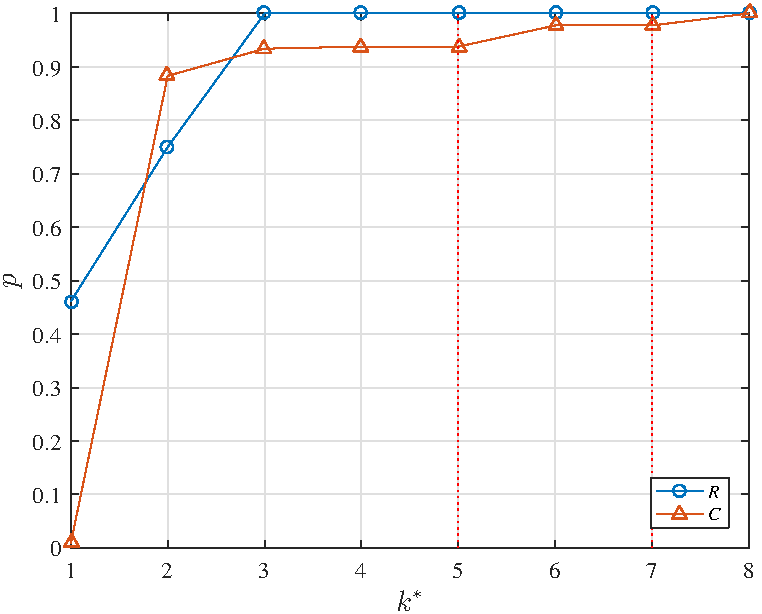
\includegraphics[width=\oneimage]{Correct_Ratio.pdf}
\end{minipage}
\setlength{\abovecaptionskip}{6pt} %调整图片标题与图距离
\setlength{\belowcaptionskip}{12pt} %调整图片标题与下文距离
\caption{示例单图}
\label{fig:ratio}
\end{figure}
引用图\ref{fig:ratio}。
\subsection{多图}
如果一个图由两个或两个以上分图组成时,各分图分别以(a)、(b)、(c)……作为图序,并须有分图名,分图名直接列在各自分图的正下方,主图名列在所有分图的下方正中。

\begin{figure}[!htb]
\centering
\begin{minipage}[t]{\twoimage}
\centering
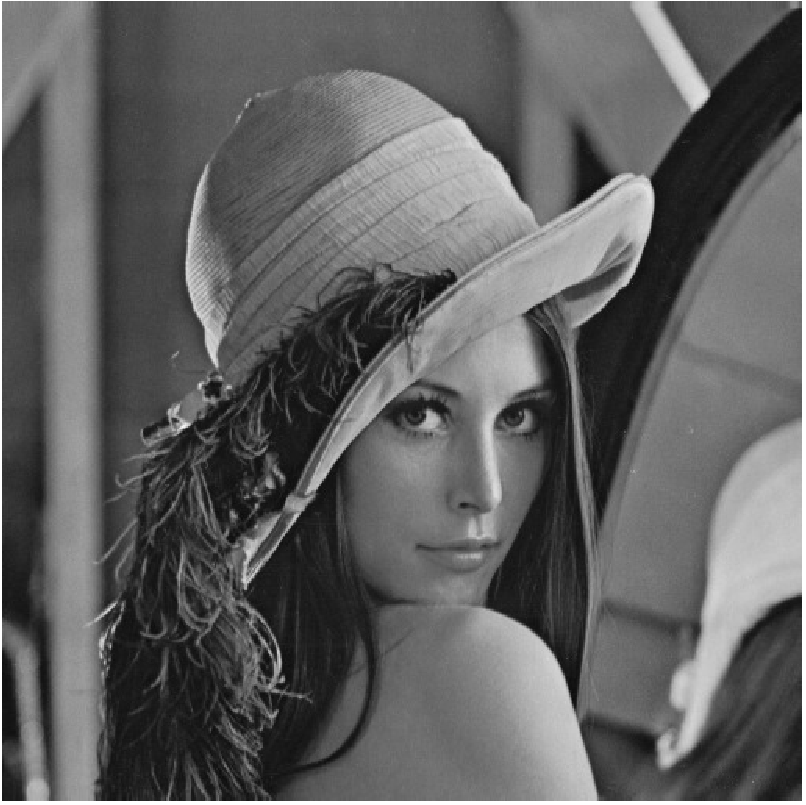
\includegraphics[width=\twoimage]{Lenna.pdf}
{\songti\zihao{5} (a)子图1}
\end{minipage} \hspace{4pt}
\begin{minipage}[t]{\twoimage}
\centering

\includegraphics[width=\twoimage]{Lenna_e.pdf}
{\songti\zihao{5} (b)子图2}
\end{minipage}
\setlength{\abovecaptionskip}{6pt} %调整图片标题与图距离
\setlength{\belowcaptionskip}{12pt} %调整图片标题与下文距离
\caption{ 示例多图}
\label{fig:APairPlaintext}
\end{figure}

\section{表格}
表题:中文字体为宋体,西文字体为Times New Roman,五号,加粗,居中无缩进,段前12磅,段后6磅,单倍行距。表序与表名之间空一格,表名中不允许使用标点符号,表名后不加标点。

表注或数据来源说明:中文字体为宋体,西文字体为Times New Roman,小五号,两端对齐,首行缩进2字符,段前0行,段后0行,固定值20磅。

\begin{table}[!htb]
\centering
\setlength{\abovecaptionskip}{12pt} %调整表格标题与上文距离
\setlength{\belowcaptionskip}{6pt} %调整表格标题与表距离

\caption{ 示例表}
\label{tb:blocksize}
\begin{tabular}{c|ccc}  \hline
\diagbox{ $q_1$ }{ $q_2$ }    & 0      & 1       & 2       \\ \hline
  0 & (8,8)  & (8,16)  & (8,32)  \\
  1 & (16,8) & (16,16) & (16,32) \\
  2 & (32,8) & (32,16) & (32,32) \\ \hline
\end{tabular}
\end{table}

\section{伪代码}
算法\ref{qsort}:

\begin{algorithm}[H]\label{qsort}
    \SetAlgoLined
    \KwData{this text}
    \KwResult{how to write algorithm with \LaTeX2e }
    initialization\;
    \While{not at end of this document}{
        read current\;
        \eIf{understand}{
            go to next section\;
            current section becomes this one\;
        }{
            go back to the beginning of current section\;
        }
    }
    \caption{How to write algorithms}
\end{algorithm}

\section{公式排版}
公式数量超过1个即应编号,并将编号置于括号内,如果数量较少,全篇统一编号,如(1),如数量较多,则应分章编号,如(1-1),公式编号右端对齐,与公式间以...连接。包含公式的段落行间距可设置为最小值20磅,以保证公式完全显示。

已知$a+b=c$,那么

\begin{equation}\label{eq:aplusb}
\usetagform{dots}
  a=c-b.
\end{equation}

来看公式\ref{eq:amultib}:

\begin{equation}\label{eq:amultib}
  a*b=c.
\end{equation}

证明:

\begin{proof}
  地球是围着太阳转的
\end{proof}

$\pm$ 

% \chapter{标题}
% \section{标题}
% \subsection{标题}


% \chapter{标题}
% \section{标题}
% \subsection{标题}


% \chapter{结论}
%----------------------------------------prereference---------------------------
\CTEXsetup[format={\centering\songti\bfseries\zihao{3}},name={},number={\arabic{chapter}}]{chapter}
\CTEXsetup[beforeskip={24pt},afterskip={18pt}]{chapter}
%----------------------------------------reference---------------------------
\setlength{\bibsep}{1pt}
\def\bibfont{\songti\zihao{5}}
\phantomsection
\addcontentsline{toc}{chapter}{参考文献}

\bibliography{reference/ref} 
参考文献另起一页,宋体三号,加粗,居中对齐,无缩进,大纲级别1级,段前24磅,段后18磅,固定值20磅。

中文字体为宋体,西文字体为Times New Roman,五号,两端对齐,编号1-9的文献悬挂缩进0.6厘米,编号10-99的文献悬挂缩进0.74厘米,编号100以上的文献悬挂缩进0.9厘米(以保证文献内容相对于编号左对齐),段前0行,段后0行,1.5倍行距。
参考文献和注释格式需保证全篇统一。

%----------------------------------------thanks------------------------------
\chapter*{致~~~~谢}
\phantomsection
\addcontentsline{toc}{chapter}{致谢}
致谢二字中间空两个汉字空格或4个半角空格,宋体三号,加粗,居中对齐,无缩进,大纲级别1级,段前24磅,段后18磅,固定值20磅。另起一页。

中文字体为宋体,西文字体为Times New Roman,小四号,大纲级别正文文本,两端对齐,首行缩进2字符,段前0行,段后0行,固定值20磅。
%----------------------------------------preAppendix------------------------------
\CTEXsetup[format={\songti\bfseries\zihao{3}},name={},number={\arabic{chapter}}]{chapter}
\CTEXsetup[beforeskip={24pt},afterskip={18pt}]{chapter}
%----------------------------------------Appendix------------------------------
\chapter*{附录A}
\phantomsection
\addcontentsline{toc}{chapter}{附录A}
附录:含论文检测报告、计算机程序、译文及原件等,依序用大写正体A,B,C……编序号,如:附录A,每个附录另起一页。附录中的图、表、式等另行编序号,与正文分开,也一律用阿拉伯数字编码,但在数码前冠以附录序码,如:图A1;表B2;式(B3)等。
附录二字中文字体为宋体,西文字体为Times New Roman,三号,加粗,大纲级别1级,两端对齐,首行无缩进,段前24磅,段后18磅,固定值20磅。

附录内容:中文字体为宋体,西文字体为Times New Roman,五号,大纲级别正文文本,两端对齐,首行缩进2字符,段前0行,段后0行,固定值20磅。

% \chapter*{附录B}
% \phantomsection
% \addcontentsline{toc}{chapter}{附录B}

\end{document} 